\section{Crafting Systems}


\subsection{Gear Crafting}

\paragraph{Overview}
The Gear Crafting System combines deterministic player-driven modification (Affixes) with random initial base generation (Implicits). 
Each gear item is defined by its \textbf{Gear Type} (Head, Chest, Leg, Boots, Gloves, Amulet) and can contain:
\begin{itemize}
	\item Up to \textbf{N Implicits} (rolled automatically on creation)
	\item Up to \textbf{M Affixes} (player-crafted and upgradable)\\
\end{itemize}

Each mechanic type has its own input/output schema, cost structure, and scaling formula.
All crafting transactions are atomic (no partial resource loss).\\
Access to specific crafting mechanics (Infuse, Re-Infuse, Tempering, Over-Tempering) is gated by the Crafting Research Tree (see Section~\ref{subsec:research-system}).
Early game only basic recipes are available; advanced mechanics unlock gradually.\\

Ingredients are always Materials (Parts, Remains). 
Currencies are account-wide resources (e.g. Gold, Crystals) and are not stored in the item inventory.

\vspace{0.5em}
\noindent
\textbf{Design Goal:} Create meaningful player agency through controlled randomness and resource-driven progression.
\vspace{1em}

% =============================================================
\subsubsection{Mechanic I – Basic Crafting (Gear Recipes)}

\paragraph{Purpose}
Convert raw materials (and optional boosters) into finished base gear items.

\paragraph{Sequence}

\begin{minipage}[t]{0.48\textwidth}
	\vspace{0pt}\centering
	Flow: Basic Gear Crafting
	\resizebox{\linewidth}{!}{
		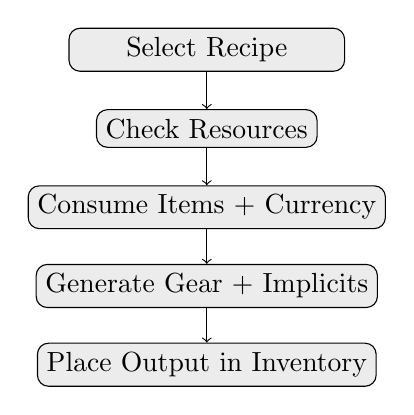
\begin{tikzpicture}
			\node[draw,rounded corners,fill=gray!15,minimum width=3.5cm] (select) {Select Recipe};
			\node[draw,rounded corners,fill=gray!15,below of=select] (check) {Check Resources};
			\node[draw,rounded corners,fill=gray!15,below of=check] (consume) {Consume Items + Currency};
			\node[draw,rounded corners,fill=gray!15,below of=consume] (generate) {Generate Gear + 	Implicits};
			\node[draw,rounded corners,fill=gray!15,below of=generate] (output) {Place Output in 	Inventory};
			
			\path[->] (select) edge (check)
			(check) edge (consume)
			(consume) edge (generate)
			(generate) edge (output);
		\end{tikzpicture}%
	}
\end{minipage}

\paragraph{Input / Output Schema}
\begin{center}
	\begin{tabular}{|l|l|}
		\hline
		\textbf{Element} & \textbf{Description / Constraints} \\ \hline
		Ingredients & Up to 4 \textbf{Materials} (Parts / Remains, each with quantity). \\
		Booster    & Max 1 optional \textbf{Booster Material} (typically high-tier Remains). \\
		Currency   & Any number of \textbf{Currencies} (Gold, Crystals or similar). \\
		Output     & 1 Gear \textbf{item}. \\
	\end{tabular}
\end{center}

\paragraph{Cost Structure}

\begin{itemize}
	\item Base cost determined by item rarity and recipe complexity.
	\item Optional booster adds both cost and potential reward.
	\item Currency cost acts as sink to regulate player economy.
\end{itemize}

\subparagraph{Cost Scaling}
...

\paragraph{Booster Effect}
based on Rarity/Qualtiy and Quantity of the used Booster-Material the output is modified.
\begin{center}
	\begin{tabular}{|l|l|l|}
		\hline
		\textbf{Parameter} & \textbf{Symbol / Range} & \textbf{Description} \\ \hline
		Tier Boost per Unit & $f_1(q)$ & Adds virtual tier levels to implicits. \\
		Roll Bias per Unit & $f_2(q)$ & Shifts random roll toward max value. \\
		Caps & $\text{cap}_T, \text{cap}_B$ & Hard caps for both effects. \\
		Diminishing Curve & $D(q)$ & Function for diminishing returns. \\ \hline
	\end{tabular}
\end{center}

\paragraph{Implicits}

Implicits and base rolls per Tier \\
\begin{tabular}{|l|l|l|l|c|c|c|}
	\hline
	\textbf{Kurzname} & \textbf{Implicit Effekt} & \textbf{Type} & \textbf{Tag} & \textbf{T1 roll} & \textbf{T2 roll} & \textbf{T3 roll} \\
	\hline
	DMG\%            & increased damage                & \%    & damage  & 5--10   & 10--15  & 15--25 \\
	Thorns           & to thorns                       & flat  & damage  & 1--5    & 5--7    & 7--12  \\
	Phys+            & to phys damage                  & flat  & damage  & 1--5    & 5--7    & 7--12  \\
	Elem+            & to elemental damage             & flat  & damage  & 1--5    & 5--7    & 7--12  \\
	\hline
	Armor\%          & increased armor                 & \%    & defence & 5--10   & 10--15  & 15--25 \\
	Res\%            & increased elemental resistance  & \%    & defence & 5--10   & 10--15  & 15--25 \\
	Dodge\%          & increased dodge chance          & \%    & defence & 5--10   & 10--15  & 15--25 \\
	Barrier         & increased barrier                & \%  & defence & 5--10   & 10--15  & 15--25 \\
	Armor+           & to armor                        & flat  & defence & 30--60  & 60--100 & 100--150 \\
	MaxBarrier+      & to max barrier                  & flat  & defence & 30--60  & 60--100 & 100--150 \\
	\hline
	Life\%           & increased life                  & \%    & life    & 5--10   & 10--15  & 15--25 \\
	MaxLife+         & to max Life                     & flat  & life    & 20--40  & 40--75  & 75--120 \\
	\hline
	Rarity\%         & increased item rarity           & \%    &  & 5--7    & 7--10   & 10--15 \\
	Speed\%           & increased movement speed        & \%    & speed   & 10--15  & 15--25  & 25--40 \\
	\hline
\end{tabular}

\par
weight rolls of implicit for each geartype\\

\begin{tabular}{|l|r r r r r r|}
	\hline
	\textbf{Stat} & \textbf{Head} & \textbf{Chest} & \textbf{Gloves} & \textbf{Legs} & \textbf{Boots} & \textbf{Amulet} \\
	\hline
	DMG\%        & 100 &  50 & 300 & 100 &  50 & 500 \\
	Thorns       &   0 & 100 &  50 & 100 & 300 &   0 \\
	Phys+        & 100 &  50 & 300 & 100 &  50 & 300 \\
	Elem+        & 300 &  50 & 100 & 100 &  50 & 300 \\
	Armor\%      & 100 & 500 &  50 & 300 & 100 & 100 \\
	Res\%        & 300 & 500 &   0 & 300 &  50 & 100 \\
	Dodge\%      & 300 & 100 &  50 & 500 & 200 &  50 \\
	Barrier\%    & 300 & 300 & 100 & 100 &  50 & 200 \\
	Armor+       & 100 & 500 &  50 & 100 & 100 &  50 \\
	MaxBarrier+  & 100 & 300 & 100 & 100 & 100 &  50 \\
	Life\%       & 100 & 500 &  50 & 100 &  50 & 200 \\
	MaxLife+     & 100 & 500 &  50 & 100 & 100 &  50 \\
	Rarity\%     &  50 &  25 &  50 &  50 & 100 & 100 \\
	Speed\%      &   0 &   0 &   0 &   0 & 750 &   0 \\
	\hline
	\textbf{sum} & 1950& 3475& 1250& 2050& 2050& 2000 \\
	\hline
\end{tabular}


\vspace{1em}
% =============================================================
\subsubsection{Mechanic II – Upgrade / Affix Crafting}

\paragraph{Purpose}
Allows the player to add new affixes, upgrade existing tiers, or perform one reroll on a designated slot.

\paragraph{Sequence}

\begin{minipage}[t]{0.48\textwidth}
	\vspace{0pt}\centering
	Flow: Add Affix
	\resizebox{\linewidth}{!}{
		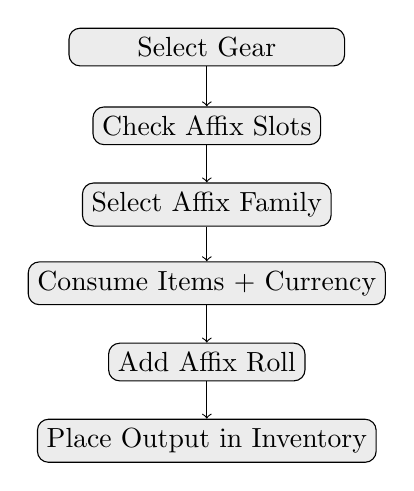
\begin{tikzpicture}
			\node[draw,rounded corners,fill=gray!15,minimum width=3.5cm] (select) {Select Gear};
			\node[draw,rounded corners,fill=gray!15,below of=select] (check) {Check Affix Slots};
			\node[draw,rounded corners,fill=gray!15,below of=check] (select2) {Select Affix Family};
			\node[draw,rounded corners,fill=gray!15,below of=select2] (consume) {Consume Items + Currency};
			\node[draw,rounded corners,fill=gray!15,below of=consume] (generate) {Add Affix Roll};
			\node[draw,rounded corners,fill=gray!15,below of=generate] (output) {Place Output in Inventory};
			
			\path[->] (select) edge (check)
			(check) edge (select2)
			(select2) edge (consume)
			(consume) edge (generate)
			(generate) edge (output);.
		\end{tikzpicture}%
	}
\end{minipage}\hfill
\begin{minipage}[t]{0.48\textwidth}
	\vspace{0pt}\centering
	Flow: Reroll Affix
	\resizebox{\linewidth}{!}{
		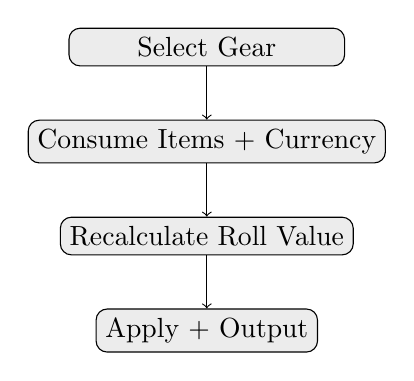
\begin{tikzpicture}[node distance=1.2cm]
			\node[draw,rounded corners,fill=gray!15,minimum width=3.5cm] (select) {Select Gear};
			\node[draw,rounded corners,fill=gray!15,below of=select] (consume) {Consume Items + Currency};
			\node[draw,rounded corners,fill=gray!15,below of=consume] (recalc) {Recalculate Roll Value};
			\node[draw,rounded corners,fill=gray!15,below of=recalc] (save) {Apply + Output};
			\path[->] (select) edge (consume)
			(consume) edge (recalc)
			(recalc) edge (save);
		\end{tikzpicture}
	}
\end{minipage}


\paragraph{Input / Output Schema}
\begin{center}
	\begin{tabular}{|l|l|}
		\hline
		\textbf{Element} & \textbf{Description / Constraints} \\ \hline
		Base Item & Gear item with available affix slots. \\
		Materials & Crafting reagents depending on action. \\
		Currency & Gold or rare currencies. \\
		Output & Mutated item (same ID, new affix or tier). \\ \hline
	\end{tabular}
\end{center}

\paragraph{Cost Structure}

\begin{itemize}
	\item \textbf{Add Affix:} base cost plus weighted RNG PickSize (2--4).    
	\item \textbf{Reroll:} 1 time per item: high base cost that scales further with the item tier 
\end{itemize}

\subparagraph{Cost Scaling}

tbd

\paragraph{Affix Pools}

\subparagraph{Core Pool}
\begin{center}
	\begin{tabular}{|l|l|l|c c c|}
		\hline
		\textbf{Affix effect} & \textbf{type} & \textbf{tag} & \textbf{T1 roll} & \textbf{T2 roll} & \textbf{T3 roll} \\
		\hline
		to STR                                & flat & attribute & 3--7   & 7--15   & 15--20  \\
		to DEX                                & flat & attribute & 3--7   & 7--15   & 15--20  \\
		to CON                                & flat & attribute & 3--7   & 7--15   & 15--20  \\
		to INT                                & flat & attribute & 3--7   & 7--15   & 15--20  \\
		to WIL                                & flat & attribute & 3--7   & 7--15   & 15--20  \\
		\hline
		increased crit chance                 & \%   & crit      & 10--15 & 15--25  & 25--40  \\
		increased crit dmg                    & \%   & crit      & 30--60 & 60--100 & 100--150 \\
		\hline
		increased phys damage                 & \%   & damage    & 20--40 & 40--75  & 75--120 \\
		increased elemental damage            & \%   & damage    & 20--40 & 40--75  & 75--120 \\
		\hline
	\end{tabular}
\end{center}

\subparagraph{Defensive Pool}
\begin{center}
	\begin{tabular}{|l|l|l|c c c|}
		\hline
		\textbf{Affix effect} & \textbf{type} & \textbf{tag} & \textbf{T1 roll} & \textbf{T2 roll} & \textbf{T3 roll} \\
		\hline
		increased all resistance (phys/elem)  & \%   & defence   & 10--15 & 15--25  & 25--40  \\
		reduced DoT duration                  & \%   & defence   & 10--15 & 15--25  & 25--40  \\
		gain \% reflect equal to dodge rating & \%   & defence   & 20--40 & 40--75  & 75--120 \\
		to barrier regen per second           & flat & defence   & 3--7   & 7--15   & 15--20  \\
		reduce barrier recharge delay         & \%   & defence   & 10--15 & 15--25  & 25--40  \\
		\hline
		\% dmg taken recouped as life         & \%   & life      & 1--4   & 4--8    & 8--12   \\
		leech damage as life                  & \%   & life      & 1--4   & 4--8    & 8--12   \\
		to life regen per second              & flat & life      & 5--10  & 10--25  & 25--40  \\	
		\hline
	\end{tabular}
\end{center}

\subparagraph{Synergy Pool}
\begin{center}
	\begin{tabular}{|l|l|l|c c c|}
		\hline
		\textbf{Affix effect} & \textbf{type} & \textbf{tag} & \textbf{T1 roll} & \textbf{T2 roll} & \textbf{T3 roll} \\
		\hline
		\% armor applies to all Dmg           & \%   & damage    & 10--15 & 15--25  & 25--40  \\
		\% crit chance applies to phys Dmg    & \%   & damage    & 10--15 & 15--25  & 25--40  \\
		\% dodge rating applies to thorns     & \%   & damage    & 10--15 & 15--25  & 25--40  \\
		\% Barrier applies to elem damage     & \%   & damage    & 10--15 & 15--25  & 25--40  \\
		\% phys damage penetrates armor       & \%   & damage    & 10--15 & 15--25  & 25--40  \\
		\% elem damage penetrates resistance  & \%   & damage    & 10--15 & 15--25  & 25--40  \\
		\hline
	\end{tabular}
\end{center}

\subparagraph{Utility Pool}
\begin{center}
	\begin{tabular}{|l|l|l|c c c|}
		\hline
		\textbf{Affix effect} & \textbf{type} & \textbf{tag} & \textbf{T1 roll} & \textbf{T2 roll} & \textbf{T3 roll} \\
		\hline
		increased melee skill power           & \%   & skill     & 20--40 & 40--75  & 75--120 \\
		increased projectile speed            & \%   & skill     & 20--40 & 40--75  & 75--120 \\
		increased area of effect              & \%   & skill     & 20--40 & 40--75  & 75--120 \\
		increased ranged skill power          & \%   & skill     & 20--40 & 40--75  & 75--120 \\
		increased range                       & \%   & skill     & 20--40 & 40--75  & 75--120 \\
		increased pierce chance               & \%   & skill     & 20--40 & 40--75  & 75--120 \\
		\hline
		increased cast speed                  & \%   & speed     & 20--40 & 40--75  & 75--120 \\
		reduced cooldown                      & \%   & speed     & 10--15 & 15--25  & 25--40  \\
		\hline
		increased item rarity                 & \%   &    & 10--15 & 15--25  & 25--40  \\
		\hline
	\end{tabular}
\end{center}


\paragraph{Reroll Affix}

\begin{itemize}
	\item Only one slot per item can be rerolled
	\item slot is chosen randomly
	\item Rerolls the Affix effect
	\item no duplicate of existent Affixes
	\item the more Affixes are on the item, the smaller the Reroll-Range of which Affix will be rolled
	\item relativley high base cost, but no Sclaing, since 1 time per item
\end{itemize}


\vspace{1em}
% =============================================================
\subsubsection{Mechanic III – Hardening (Tier Enhancement)}

\paragraph{Purpose}
A late-game mechanic that permanently increases item potential through tier reinforcement and needs a late-game research to be finsihed.

\paragraph{Sequence}

\begin{center}
	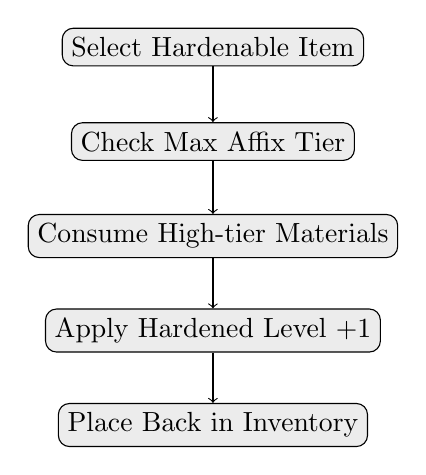
\begin{tikzpicture}[node distance=1.2cm]
		\node[draw,rounded corners,fill=gray!15,minimum width=3.5cm] (select) {Select Hardenable Item};
		\node[draw,rounded corners,fill=gray!15,below of=select] (check) {Check Max Affix Tier};
		\node[draw,rounded corners,fill=gray!15,below of=check] (consume) {Consume High-tier Materials};
		\node[draw,rounded corners,fill=gray!15,below of=consume] (enhance) {Apply Hardened Level +1};
		\node[draw,rounded corners,fill=gray!15,below of=enhance] (output) {Place Back in Inventory};
		\path[->] (select) edge (check)
		(check) edge (consume)
		(consume) edge (enhance)
		(enhance) edge (output);
	\end{tikzpicture}
\end{center}

\paragraph{Input / Output Schema}
\begin{center}
	\begin{tabular}{|l|l|}
		\hline
		\textbf{Element} & \textbf{Description / Constraints} \\ \hline
		Base Item & Crafted item with maxed affixes. \\
		Materials & Rare tier-enhancing reagents. \\
		Currency & High-end currency cost (flat + exponential). \\
		Output & Same item with upgraded ``Hardened'' property. \\ \hline
	\end{tabular}
\end{center}

\paragraph{Hardening Tiers}
\begin{center}
	\begin{tabular}{|c|c|c|c|}
		\hline
		\textbf{Level} & \textbf{Cost Multiplier} & \textbf{Effect} & \textbf{Notes} \\ \hline
		1 & x1 & increase roll within the tier &  \\ 
		2 & x2 & increase roll within the tier &  \\ 
		3 & x4 & +1 Tier  &  \\ 
		4 & x5 & increase roll within the tier &  \\ 
		5 & x6 & increase roll within the tier &  \\ 
		6 & x12 & +1 Tier &  \\
		7 & x13 & increase roll within the tier &  \\
		8 & x14 & increase roll within the tier &  \\
		9 & x28 & +1 Tier &  \\ 
		10& x29 & increase roll within the tier & \\
		11& x30 & increase roll within the tier & \\
		12& x60 & Overroll (over Max) & extreme high cost for late endgame\\ \hline
	\end{tabular}
\end{center}

\paragraph{Cost Structure}

\begin{itemize}
	\item Each hardening level multiplies base material and currency cost.
	\item Rare materials required (e.g., Essence, Soul Alloy).
\end{itemize}

\subparagraph{Cost Scaling}

see Cost Multiplicator in Hardening Tiers


\vspace{1em}
% =============================================================
\subsubsection{General Validation Rules}

\begin{itemize}
	\item Recipes must define $\leq 4$ ingredients and $\leq 1$ booster.
	\item All costs non-negative; zero costs invalid.
	\item ItemBaseDef must specify GearType and AllowedPools.
	\item Atomic transactions: no partial resource consumption.
	\item Rollback mandatory on any failure path.
\end{itemize}


\subsection{Module Crafting}

%TODO: complete. here are just some general ideas
\textit{- Idea: not crafting but Exchange (cores and remains and other currency) - researchable }\\
- Modules are crafted from Parts or remains and a special boss mob drops (cores?)\\
- cores come in different eleemtns\\
- the used "core" defines the damage type of the module:\\

\begin{tabular}{l l}
	\textbf{Core Type} & \textbf{Damage Type} \\
	\hline
	Kinetic  & Physical      \\
	Blazing  & Fire          \\
	Glacial  & Cold          \\
	Static   & Lightning     \\
	Venomous & Poison        \\
	Aetheric & Arcane        \\
	Infernal & Dark/Demonic  \\
	Radiant  & Holy          \\
	\hline
\end{tabular}


\subsection{Rune Crafting}
Future Idea for endgame progression of skills/heroes
